\documentclass[../main.tex]{subfiles}

\begin{document}
\chapter{Combinatorial Search}
What is the most straightforward way to solve problems? We form it as a search problem in \textit{search space}--a simple example is to enumerate all possibilities--and search among them what we need. We introduce the general searching strategies and learn some math--combinatorics that we strongly need. 
\section{Introduction}
Combinatorial search problems consists of $n$ items and a requirement to find a solution, i.e., a set of $L < N$ items that satisfy specified conditions or constraints. For example, a sudoku problem where a $9\times 9$ grid is partially filled with number between 1 and 9, fill the empty spots with numbers that satisfy the following conditions:
\begin{figure}[!ht]
    \centering
    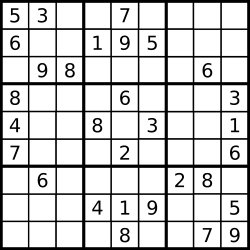
\includegraphics[width= 0.35\columnwidth]{fig/250px-Sudoku-by-L2G-20050714.png}
    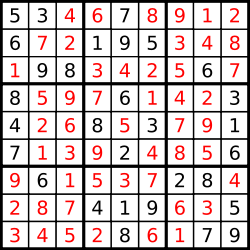
\includegraphics[width= 0.35\columnwidth]{fig/250px-Sudoku-by-L2G-20050714_solution.png}
    \caption{Example sudoku puzzle and its solution}
    \label{fig:backtrack_puzzle_1}
\end{figure}
\begin{enumerate}
    \item Each row has all numbers form 1 to 9.
    \item Each column has all numbers form 1 to 9.
    \item Each sub-grid ($3 \times3$) has all numbers form 1 to 9.
\end{enumerate}
The sudo problem together with one possible solution is shown in Fig.~\ref{fig:backtrack_puzzle_1}. In this case, we have $81$ items, and we are required to fill 51 empty items with the above three constraints. Combinatorial search in computer science mainly studies algorithms that solve exponential or even NP-hard problems, such as:
\begin{enumerate}
    \item Constraint Satisfication Problems (CSP) such as sudoku, N-queen, and so on.
    \item Optimization problems such as Travel Salesman Problems (TSP) and knapsack problems. 
\end{enumerate}

\paragraph{Techniques} From Chapter Discreet Programming, we have learned the basics of enumerative combinatorics, including counting principles and knowledge on permutations, combinations, partitions, subsets, and subsequences. Combinatorial search builds on top of this subject, and together through the technique in computer science which is called ``backtracking'', it is able to enumerate the search space   and find the solution effectively and efficiently with necessary speedup methods. 



\paragraph{Search Problem} A search problem is defined as a problem that there is an algorithmic way to verify its answer. Finding a certain integer on an array of integers is a simplest example. 

For the searching on input instance with a peculiar data structure, the search space itself is all items in this data structure, searching in this space is a simply applying searching strategies specified by data structure and situation, which we have already covered in Chapter. Searching on Data Structures. However, for problems that are not explicitly a searching on a data structure, to form it as a search problem, we need to define \textit{state}, \textit{state space}, and \textit{goal test}. 

\subsubsection{State, State Space, and Goal Test} What is a state? A state can be imagined as a container that holds all information of it. A state Space is a set of all possible states in a problem domain. For a discrete problem, this set will be finite, which is good news. We use $S$ to make the state, and $V_s$ to mark the state space. Let's look at an example about subarray.
\paragraph{Example: Subarray Problem (L560)} Given an array of integers and an integer $t$, find the total number of continuous subarrays whose sum equals to $t$.
\begin{lstlisting}[numbers=none]
a=[1,1,1], t=2
Return 2
\end{lstlisting}
In this question, we care about information about subarray and its sum,  state here can be further named as `a subarray start at index $i$ and end at index $j$, and its sum is $value$'. We use $a_{ij}, i\leq j, j\in[0,n-1]$ to make a subarray, and $s_{ij}=v$ a state. Simple math tells us we have total number of $n+(n-1)+(n-2)+...+1=\frac{n\times(n+1)}{2}$ subarries, which makes $|V_s|$. A goal test can be set as ``checking if any subarray has a sum value same as $t$''. Beside, there should always be an \textit{initial state}, wherein this case it should be an empty array with value of $0$, we mark it as $\empty$.

So far, we can use the Python code to solve this problem by generating all states and do goal testing:
\begin{lstlisting}[language=Python]
# Generate all subarries
def naive_subarray_sum(a, t):
  if not a:
    return 0
  n = len(a)
  ans = 0
  # simple enumeration
  for i in range(n):
    for j in range(i, n):
      # define the state and compute its value
      s_ij = 0 
      for k in range(i,j+1):
        s_ij += a[k]
      # goal test
      if s_ij == t:
        ans += 1
  return ans  
\end{lstlisting}

\subsubsection{State Transfer Model} The problem of the above implementation is that we did just blindly compute each sate, but never think about connections between state. A easy one that comes to our mind is $s_{ij}=s_{ij-1}+a_j$. From $s_{ij-1}$ to $s_{ij}$ we need only one addition; whereas in our previous way, we treated the states independently and spend $j-i$ additions to compute its state. This is called a \textit{state transfer model}. With this prior knowledge, we can completely cut off the innermost \texttt{for} loop. We can draw the state transfer model as a graph, where there will be an arc $a\xrightarrow{}b$ if state $a$ can be converted to state $b$:
\begin{lstlisting}[numbers=none]
[]->a_00->a_01->a_02
[]->a_11->12
[]->a_22
\end{lstlisting}
The code can be shown:
\begin{lstlisting}[language=Python]
# State transfer model
def state_transfer_subarray_sum(a, t):
  if not a:
    return 0
  n = len(a)
  ans = 0
  # simple enumeration
  for i in range(n):
    s_ij = 0
    for j in range(i, n):
      # a sate only depends on its previous state
      s_ij = s_ij + a[j] 
      if s_ij == t:
        ans += 1
  return ans 
\end{lstlisting}
The state transfer actually used the \textit{reduce and conquer} principle. Each state is considered as a subproblem of the original problem. And a larger problem can be reduced into a set of smaller subproblems. The state transfer model is equivalently using this method. 
\subsubsection{Reduce the State Space Further} There actually has a even better way to do this. We can define a state as ``the number of subarray that has sum equals to $t$ in an array of $a_{0,j}$, and we have the sum of the whole array as $sum$'', we short it for $s(j,sum,count)$. We need to use two data strcutures to track this state $dp[j]=count$ and $sum[j]$. In this definition, there is only one variable $j$ to indicate the total number of states. Now, what is the recurrence relation between $dp_j$ and $dp_{j-1}$? There are two options for the item $a_j$. First, it can be part of a qualified subarray, which means we need to find a previous state say $0-k$, then our current state is $0,1,..., k, k+1, ..,j$. We need a previous state $k$ which has $sum[k]=sum_[j]-t$. If we know how many such previous subproblem exist as $c$, our $dp[j]=c$. Second, when $a_j$ is not considered, we just simply has $dp[j]=dp[j-1]$. Sum up both cases: $dp=c+dp[j-1]$. The problem here become how to find $c$ efficiencly, and possibly just constant operations. We can save information $sum$ of a state into a hasing table (dictionary), which uses $sum$ as key and $c$ as values. The Python code is:
\begin{lstlisting}[language=Python]
from collections import defaultdict
def subarraySum(a, t):
    """
    :type nums: List[int]
    :type t: int
    :rtype: int
    """
    sum_i = 0
    dict = defaultdict(int) #sum 0, count = 0
    dict[0] = 1
    dp = [0]*(len(a)+1)
    for idx, v in enumerate(a):
        sum_i += v
        if sum_i - t in dict:
            dp[idx+1] = dict[sum_i-t] + dp[idx]
        else:
            dp[idx+1] = dp[idx]
        dict[sum_i] += 1

    return dp[-1]
\end{lstlisting}
\subsubsection{Problem Solving Guideline***} Heretofore, we learned the five key components of formulating a search problem: state, initial state, state space, state transfer, and goal test. 

\paragraph{Exhaustive Search} To solve a search problem, there are some directions:
\begin{itemize}
\item if it is explicit data structure, apply particular searching strategy will do the problem easily!
\item if it is implicit data structure, we generate and save our state such as in our example where enumerate the state and compute its values in \texttt{s\_{ij}}. This also depends on the data structure that the state space forms. This chapter focuses on solving problems in this stage via enumeration and goal test. To be able to enumerate and count the size of the state space, we need combinatorics and its implementation with depth-first search based \textbf{``backtracking''} technique.   
\end{itemize}
\paragraph{Optimization via Searching} To optimize a search problem within a search strategy, we need to prune as much  unqualified or unnecessary branch as possible. We introduce two ways:
\begin{itemize}
    \item Branch and Prune: This method prunes the unqualified branches with constraints of the problems. This is usually applied to solve constraint restricted problems (CSPs), and backtracking is a top technique to do it.  
    \item Branch and Bound: This method prunes unnecessary branches via comparing an estimation of this node with a found global best solution to see; if the estimation will never lead us to a better solution, we cut off this branch. Either backtracking or best-first search can be applied. This technique can be applied to solve a general optimization problems, such as Travel Salesman Problems (TSP), knapsack problems, and so.
\end{itemize}
Therefore, these searching and prunning techniques are  widely applied to solve combinatorial problems, constraint restricted problems (CSPs), and optimization problems.

\paragraph{Other Optimization Techniques}
There are three directions to get better accuracy, which are trailers for the remaining chapters sitting in this part. So, DONNOT worry if you do not understand it all, read it first and come back to check it out later after you have learned these chapters. 
\begin{itemize}
\item Reducing the cost of computing each state by finding connection between states. Such connections appears as an arc in the state transfer graph and can usually be obtained by \textbf{Reduce and Conquer} method which reduce problems to subproblems and uses recurrence relation to denote its conversion. We will detail this method in Chapter. \ref{chapter_divide_conquer}. The recurrence relation guarantees lower cost to get a state from a previous state. We showed the example of computing \texttt{s\_{ij}} in the section of State Transfer Model. And here the time complexity is reduced from $O(n^3)$ to $O(n^2)$.
\item Reducing the state space, which might requires us to define the state in another way.  We have seen in the above section, we further reduced the cost to $O(n)$.
\item If the recurrence relation shows some states  appear in the search tree multiple times or in the graph there exist vertices that have indegree larger than 1, we can use \textbf{dynamic programming} to cut off the redundancy. Or else, we can make greedy choice via \textbf{Greedy Algorithms}.
\end{itemize}




%%%%%%%%%%%%%%%%%%%%%%Backtracking%%%%%%%%%%%%%%%%%%%%%%%%%%%%%%%%%
\section{Backtracking}

We know how to count the possibilities and how to enumerate them, manually. Time to learn how to program them efficiently. If we were thinking about iteration programming, we would encounter at least $n$ levels of \texttt{for} loops, which is not manageable and a pain to writ the code. This is where the recursion is great! The recursive method we apply here is  \textit{backtracking}. 

\paragraph{Introduction to Backtracking} Backtracking is a general problem-solving technique for finding all (or some) solutions to some computational problems, that \textit{incrementally} builds candidates to the solutions. Backtracking is all about choices and consequences. It shows the following two properties:
 \begin{enumerate}
     \item \textbf{No Repetition and Completion:} It is a systematic generating method that enumerate all possible states exactly at most once: will not miss any possible right solution but  avoids repetitions. If there is the ``correct'' solution, it is guaranteed to find. This property makes it ideal for solving combinatorial problems such as combination and permutation which requires us to enumerate all possible solutions. We focus on demonstrating this property in this section. 
    \item \textbf{Search Pruning:} Along the way of working with partial solutions, in some cases, it is possible for us to decide if they will  lead to a valid \textit{complete solution}. As soon as it is confident to judge its invalid configuration or it will not be optimal, it abandons  this \textit{partial candidate}, ``backtracks'' (return to the upper level), and reset to the upper level's state so that the search process can continue to explore the next branch to provide more efficiency.  This is called \textit{search pruning} among searching algorithms.  With search pruning
and we end up amortizely visiting each vertex less than once which is more
efficient compared with an exhaustive graph search such as DFS and BFS.  This property makes backtracking the most promising way to solve \textit{constraint satisfaction problem (CSP)}\footnote{CSPs are mathematical questions defined as a set of objects whose state must satisfy a number of constraints or limitations, visit \url{https://en.wikipedia.org/wiki/Constraint_satisfaction_problem} for more information}, where the goal is to find a set of value assignments to certain variables that will satisfy specific mathematical equations and inequations. For example,  Eight Queens puzzle, Map Coloring problem, Sudoku, Crosswords, and many other logic puzzles. We show examples in Section.~\ref{chapter_combinatorics_backtracking_csp}.
 \end{enumerate}

\paragraph{Model Backtracking}
We can model the combinatorial search solution as a vector $s = (s_0, s_1, ..., s_{n-1})$, where each $s_i$ is selected from a finite ordered set $A$. Such a vector might represent an arrangement where $s_i$ contains the i-th item of the permutation. Or in the combination problem, a boolean denotes if the i-th item is selected already. Or it can represent a path in a graph or a sequence of moves in a game. At each step in the backtracking algorithm, we try to extend the last partial solution $s = (s_0, s_1, ..., s_{k})$ by adding another event at the end. And then we testify our partial solution with the desired solution to decide to (1) either collect this partial solution; and or (2) add $s_{k+1}$ to the state; or (3) backtrack and reset to previous state and go to next branch.  The relation between partial state and its next state can be easily viewed as a recurrence relation. 





\subsection{Permutation}
In the case of permutate [1,2,3]. At first, we have three options: 1 or 2 or 3, we can get three possible partial result [1],[2],[3]. Second, we expand the option on the second position, for [1], we have option 2 and 3, we get [1,2], [1,3], same for [2]->[2,1],[2,3], for [3]->[3,1],[3,2]. At least, each partial result has only one option, we would get all permutations as: [1,2,3],[1,3,2],[2,1,3],[2,3,1],[3,1,2],[3,2,1]. We shall use a tree structure to better visualize this process. It is shown in Fig.~\ref{fig:backtrack_permutation}. 
\begin{figure}[h]
    \centering
    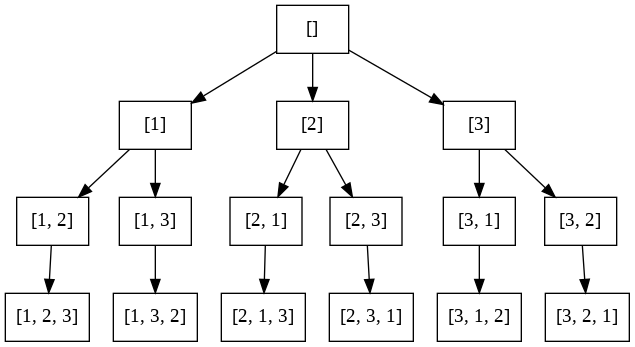
\includegraphics[width= 0.8\columnwidth]{fig/permutation.png}
    \caption{The search tree of permutation}
    \label{fig:backtrack_permutation}
\end{figure}

We start from an empty list, at this time, we have three possible options (moves), each edge represents a move, and we can go from state [], to state [1],[2],[3] with different moves. Now, how would you program to implement this? Here is one naive way: we implement it recursively as in the DFS. We use \texttt{state} to track the current partial result, \texttt{k} is used to mark the level of the recursion, it will be the same as the length of the \texttt{state}. \texttt{ans} is just used to collect the answer.
\begin{lstlisting}[language=Python]
def naive_recursion(a, state, k, ans):
  if k == len(a):
    ans.append(state[::])
    return
  for i in range(len(a)):
    if a[i] not in state:
      naive_recursion(a, state + [a[i]], k+1, ans)
\end{lstlisting}
The problem with the above implementation that line $6$ takes $O(n)$ to check if an item is valid to put into the state or not. Another thing is, each time we call \texttt{naive\_recursion}, we make a copy of \texttt{state}.This can be further avoided.

\texttt{state} is a list, when it is passed to function, it is just a pointer. However, in the case of \texttt{state + [a[i]]}, a new list is generated and passed to its recursive call. We can avoid this by appending \texttt{a[i]} at the end of \texttt{state}, and after the recursive call, we need to set the state back to its original, so that it can continue with the first \texttt{for} loop, and we can generate the next option. For example, if we are at [1], when the recursive call returned back from [1,2], if we do not set it back to [1], it can not be built to [1,3]. To avoid the second \texttt{for} loop, we can use a list of boolean \texttt{bUsed} to track which item is used. Same rule apply here, after the recursive call, we need to set its value back to False. For generality, we modify the code to generate $p(n,k)$ instead of $p(n,n)$. A better version is:
\begin{lstlisting}[language=Python]
def P_n_k(a, bUsed, state, d, k, ans):
  '''
  state start from []
  d: the level of the traversal, starts from 0
  bUsed: mark if corresponding item in a is used or not
  '''
  # reach to the last level
  if d == k:
    ans.append(state[::])
    return
  # move the state
  for i in range(len(a)):
    if not bUsed[i]:
      state.append(a[i])
      print(state)
      bUsed[i] = True
      P_n_k(a, bUsed, state, d+1, k, ans)
      bUsed[i] = False
      state.pop()
      print('backtrack: ', state)
\end{lstlisting}
Some of the process being printed out shows the process of backtracking:
\begin{lstlisting}[language=Python]
[]
[1]
[1]
[1, 2]
[1, 2]
[1, 2, 3]
backtrack:  [1, 2]
backtrack:  [1]
[1, 3]
[1, 3]
[1, 3, 2]
backtrack:  [1, 3]
backtrack:  [1]
backtrack:  []
\end{lstlisting}

\paragraph{Discussion} In this case, we can not prune any branch, because for the permutation, we need a full enumeration. 

\paragraph{Two Passes} Therefore, we can say backtracking visits these implicit vertices
in two passes: First, the forward pass to build the solution \textbf{incrementally}.
Second, the backward pass to \textbf{backtrack} to previous state. We can see within
these two passes, the \texttt{state} list is used as all vertices in the search tree, and
it start with [] and end with []. This is the core character of backtracking.

\paragraph{Time Complexity of Permutation}
In the example of permutation, we can see that backtracking only visit each state once. The complexity of this is similar to the graph traversal of $O(|V|+|E|)$, where $|V| = \sum_{i=0}^{n}{A_{n}^{k}}$, because it is a tree structure, $|E| = |v|-1$. This actually makes the permutation problem NP-hard. 

\paragraph{Space Complexity} The implementation is depth-first search, which has $O(bd)$ as the space complexity, where $b$ is branching factor and $d$ is the depth of the tree. However, in the backtracking, it even saves more space because only one state is generated at a time rather than saving all of the states belong to the same predecessor state all at once; because once it returns to the predecessor, the \texttt{for} loop there can always generate the next state. Further, in our second solution, we  reuse the state vector such as \texttt{state} in our case for enumerating all states by do modification and undo the modification once we go back to the predecessor and to generate the next successor. The slight different can be critical for problems with large state description.  
\subsection{Combination} 
\begin{figure}[!ht]
    \centering
    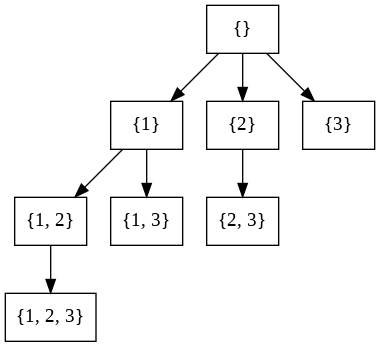
\includegraphics[width= 0.7\columnwidth]{fig/combination.png}
    \caption{The Search Tree of Combination. Change each vertex to a set instead of a list}
    \label{fig:backtrack_combination}
\end{figure}
Similarly, we try to build the combination of [1,2,3] incrementally, with initial state starting at $[]$ at the first level. Then three options give us three possible combination of $C(3,1)$: [1], [2], and [3].  For [1], we have 2 and 3, to get [1, 2], [1,3]. One option is to get exactly the same code as in permutation, but using a \texttt{set} for \texttt{state}, the second time a set appears, say  for [2], because [2,1] is the same as of [1,2] in this case, we check if it already exist. But this step can be avoided.

It makes better sense that in the search tree, we only visit each state exactly once. At [2] we need to avoid checking any item ahead of it, if you really want to use the permutation code, we can achieve the ``no repetion'' property by prunning branches: checking if one item is smaller than items in \texttt{state}, we prune the branch. From this prunning rule, you would say, wait for it, why do not we just add item that is behind the position of the very last item we added. For each recursive call, we pass it a \texttt{start} variable which starts at $0$ to point the recursive function to use items from the right location.  Because just to get the combination of 3 items out of 3 is 1 option, we get all combinations instead, a superset. This process is illustrated in Fig.~\ref{fig:backtrack_combination}. The code is as following: 
\begin{lstlisting}[language=Python]
def powerset(a, s, k, state, ans):
  # Save the state
  ans.append(state[::])
  # reach to the last level
  if k == len(a):   
    return
  for i in range(s, len(a)):
      state.append(a[i])
      powerset(a, i+1, k+1, state, ans)
      state.pop()
\end{lstlisting}
One thing I want to mention: algorithms are mostly obsessed with orders. Right ordering makes things more organized, easier to find a solution and potentially more efficient. 

\paragraph{Time Complexity of Combination}
Because backtracking ensures efficiency by visiting each state no more than once. For the combination(subset) problem, the total nodes of the implicit search graph/tree is $\sum_{k=0}^{n}C_{n}^{k} =2^n$. We can look it as another way, there are in total n objects, and each object we can make two decisions: inside of the subset or not, therefore, this makes $2^n$. 

%%%%%%%%%%%%%%%%%%%%%Others%%%%%%%%%%%%%%%%%%%%%%%%%
\subsection{Other Combinatorics}
%include all paths, subsequence, and so. 
\subsubsection{All Paths In Graph}
\label{subsec_all_paths}
% Try an example, we compute the $C_{4}^{2}$ from $[1, 2, 3, 4]$. We can get the following result. 
% \begin{figure}[h]
%     \centering
%     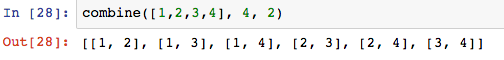
\includegraphics[width = 0.8\columnwidth]{fig/combination_rslt.png}
% \end{figure}
% Actually, the above code has redundency, each time we do not need to set the range from $s$ to $n$, we can set it to $n-k+1$ (need furthe modification). 

% If we want all the results from $k=0$ to $k=n$, we can accumulate set $k=n$, and accumulate results all the time. Actually if 
\begin{figure}[ht!]
    \centering
    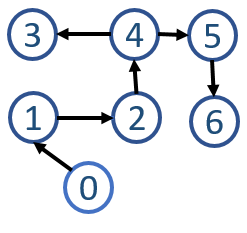
\includegraphics[width=0.4\columnwidth]{fig/all_paths.png}
    \caption{All paths from 0, include 0->1, 0->1->2,0->1->2->4, 0->1->2->4->3, 0->1->2->4->5, 0->1->2->4->5->6 }
    \label{fig:my_label}
\end{figure} 
Backtracking technique can be naturally used in graph path traversal. One example is to find all possible paths from a source to the target. One simpler occasion is when the graph has no cycles. Backtrack technique can enumerate all paths in the graph exactly once for each. 

The implementation is as follow: we still use dfs, because there has no cycles, we have no need to track the visiting state of each node. We generate the possible answer with backtracking technique through the \texttt{path} variable to track each state. 
\begin{lstlisting}[language=Python]
def all_paths(g, s, path, ans):
  '''generate all pahts with backtrack'''
  ans.append(path[::])
  for v in g[s]:
    path.append(v)
    print(path)
    all_paths(g, v, path, ans)
    path.pop()
    print(path)
\end{lstlisting}
Feed in the above network and run the following code:
\begin{lstlisting}[language=Python]
al = [[1], [2], [4], [], [3, 5], [6], []]
ans = []
path = [0]
all_paths(al, 0, path, ans)
\end{lstlisting}
With the printing, we can see the whole process, \texttt{path} changes as the description of backtrack. \begin{lstlisting}[numbers=none]
[0, 1]
[0, 1, 2]
[0, 1, 2, 4]
[0, 1, 2, 4, 3]
[0, 1, 2, 4] backtrack
[0, 1, 2, 4, 5]
[0, 1, 2, 4, 5, 6]
[0, 1, 2, 4, 5] backtrack
[0, 1, 2, 4] backtrack
[0, 1, 2] backtrack
[0, 1] backtrack
[0] backtrack
\end{lstlisting}
We can see each state, we can always have a matching backtrack state. 
\begin{bclogo}[couleur = blue!30, arrondi=0.1,logo=\bccrayon,ombre=true]{What to do if there is a cycle?} 
\end{bclogo}
\subsubsection{Subsequence}
If we observe carefully, the process of enumerating the subsequence is exactly showing the same search tree as in generateing the powerset (the better version). The only difference is in this case, the ordering actually matters. Therefore, our code will be exactly the same as we used to enumerate the powerset. 

We know the cost is $2^n$,  this is correct in the poweset too; when we are scanning the list of item there is only two options: either end up in one of the subset or not. 

\section{Prune Search Space in Backtracking}
\label{chapter_combinatorics_backtracking_csp}
So far, curious and meticulous readers might ask a question: ``Seriously, Li, I dont see the difference of the backtracking you showed me with DFS''. It's a good question, and it is worth to clarify before we move on.
\paragraph{Backtracking VS DFS} All the above examples, we used DFS to implement our backtracking algorithm. Think of backtracking as a problem-solving approach that there is a hard requirement--we force ourselves to only visit each state or configuration at most once (once for enumeration and less than once if branch pruning is applied) for consideration of efficiency, that implies that our search needs to be happening on a tree, a free tree if you want to be more specific, but we know where to start--the initial state. How to set a rule to define the free tree? This is what we engineers need to do. How to search on a free tree? That is what DFS do. Why not BFS? The space is the main issue to block us from BFS. BFS can not backtrack thus we need to save a copy of all states, not like in the DFS with backtracking we just need to dynamically append and pop from \texttt{state} we are able to experience all states.  For the case of the permutation, DFS is preferred because theoretically it took $O(\log n!)$ space used by stack (recursive call), while if use BFS, the number of vertices saved in the queue can be close to $n!$. 


\paragraph{Search Space Prunning}  In this section, we demonstrate  backtracking can be optimized via prunning search space--prunning branches in the search tree--to solve CSPs or optimization problems. Suppose we are at level 2 with state $s=(s_0, s_1)$, and if we know that this state will never lead to valid or optimal solution, we do not need to traverse through this branch but backtrack to previous state at level one. This will end up prunning half of all nodes in the search tree. We show the prunning techniques through examples and summarize them in a section.  We demonstrate the search space prunning via backtracking through two examples: TSP for branch and bound with estimates, sudoku for branch and prune with constraints.   




\subsection{Sudoku}
Sudoku problem is almost the most popular brain teaser seen in magazines, news papers or even books of its own. I bet it can be a lot effort to crack the game. In this section, we would learn how to apply backtracking and search pruning to solve this problem.
\paragraph{Sudoku Problem (L37)}
\begin{figure}[!ht]
    \centering
    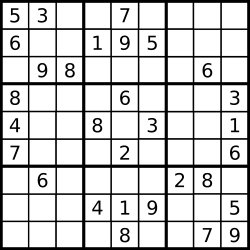
\includegraphics[width= 0.35\columnwidth]{fig/250px-Sudoku-by-L2G-20050714.png}
    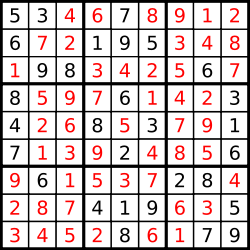
\includegraphics[width= 0.35\columnwidth]{fig/250px-Sudoku-by-L2G-20050714_solution.png}
    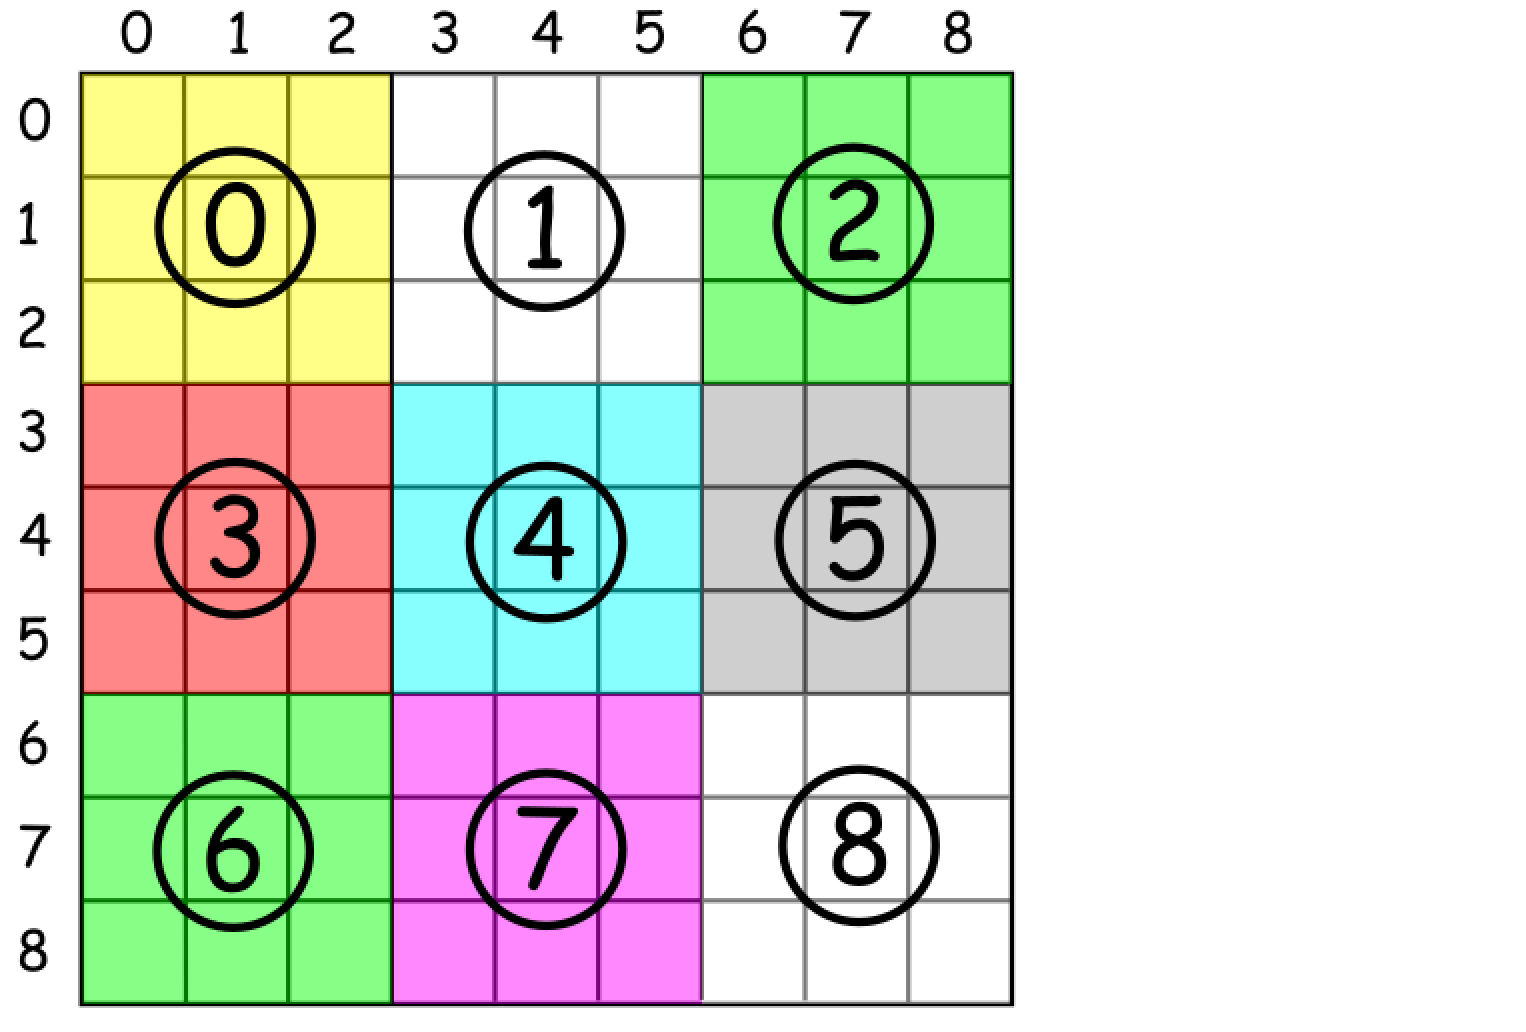
\includegraphics[width= 0.25\columnwidth]{fig/sudoku_grid.png}
    \caption{Example sudoku puzzle and its solution,( put a coloring to each block)}
    \label{fig:backtrack_puzzle}
\end{figure}
Given a  partially filled grid of size $n\times n$, completely fill the grid with number between 1 and n.  The constraint is defined as:
\begin{enumerate}
    \item Each row has all numbers form 1 to ‘n’.
    \item Each column has all numbers form 1 to ‘n’.
    \item Each sub-grid ($\sqrt{n}\times\sqrt{n}$) has all numbers form 1 to n.
\end{enumerate}
An example of a $9\times9$ sudoku problem is shown in Fig.~\ref{fig:backtrack_puzzle}.

\subsubsection{Analysis and Solution} 
\paragraph{State Space} We start by examining its state space. A state here can be defined as a $n\times n$ grid filled with numbers in range $[1,n]$. The brute force is to try 1 to n at each grid in this table, we have a state space of size $n^{n^2}$. This is beyond our current machine can handle. We apply rules: 
\begin{enumerate}
    \item Each row is essentially a permutation of integers in range $[1,n]$, this gives us $n!$ for a row, with $n$ rows, it would make the state space to $n\times n!$. 
    \item Further, each column needs to be a permutation of integers too. If we are at row 1, col 0, we would only have $n-1$ options, for position (1,1), this goes to $n-2$ options. This means our total possibility further decrease $n!+(n-1)!+...+2!+1!$. 
    \item Moreover, there is restriction in each subgrid, it becomes hard to get the exact possibility\footnote{This site \url{http://pi.math.cornell.edu/~mec/Summer2009/Mahmood/Count.html}offer some insights}. The possibility for $n=9$, is  actually  $6670903752021072936960$ which is approximately $6.671\times 10^{21}$. It is a hard problem to solve for sure. 
\end{enumerate}

 Good news, we are almost always given some prior integers in some grids, this narrows down the possibility. Applying backtracking, we first find out all empty spots, and fill up these spots recursively. An initial cost estimation can be offered, assume we have $m$ spots, and each has number of candidates $c_i$, the upper bound cost will be $c_0\times c_1\times...\times c_m$. Does the filling ordering of these empty spots matters?  For completeness, not so much; for efficiency, SURE!  Considering two approaches: one we visit these spots arbitrarily and the other we always choose spot that has the least possible candidates number to fill in (not considering the implementation right now). In the second approach, starting with less candidates can help us quickly pinpoint the right answer and cut branches that are invalid. Because the branch is easily on in the search tree, and all others are having more candidates, this pruning makes sure the branch we cut off at this stage is rewarding. Another way to think, this is essentially an greedy approach, making sure when are multiplying $c_i$ to the total cost, we are adding the least expensive ones, larger probability to guess it right, and as it accumulates, we outrun the arbitrary ones in hundreds of times faster.
 
\paragraph{Implement Sudoku with Backtracking}

In implementation, we need to track state of each row, col, and grid that what numbers it has in the process. We set aside three data structures \texttt{row\_state}, \texttt{col\_state}, and \texttt{block\_state} for this purpose so that we can validate a candidate. 
% \begin{enumerate}
%     \item Initialization: we initialize the three states and prepare data structure to track empty spots.
%     \item Backtracking and prunning: we use DFS to fill up empty spots, and each type we choose whichever in the remaining spots that has the least number of candidates. 
% \end{enumerate}


\textbf{Step 1: Initialization} We scan the whole grid shown in Fig.~\ref{fig:backtrack_puzzle} and find all empty spots that waiting for filling in.  
% From the constraints, we use the following data structures to record the state of each row, each column, and each grid.  
% \begin{lstlisting}[language=Python]
% row_state = [0]*9
% col_state = [0]*9
% grid_state = [0]*9
% \end{lstlisting}
We use (i,j) to denote the position of a grid. It correspond position $i$ in \texttt{row\_state[i]}, and $j$ in \texttt{col\_state[j]}, and \texttt{block\_state[i//3][j//3]} for corresponding sub-grid.  In this stage, we iterate through the 
\texttt{board} to record these states.
\begin{lstlisting}[language=Python]
from copy import deepcopy
class Sudoku():
  def __init__(self, board):
    self.org_board = deepcopy(board)
    self.board = deepcopy(board)
    
  def init(self):
    self.A = set([i for i in range(1,10)])
    self.row_state = [set() for i in range(9)]
    self.col_state = [set() for i in range(9)]
    self.block_state = [[set() for i in range(3)] for i in range(3)]
    self.unfilled = []

    for i in range(9):
      for j in range(9):
          c = self.org_board[i][j]
          if c == 0:
              self.unfilled.append((i, j))
          else:
              self.row_state[i].add(c)
              self.col_state[j].add(c)
              self.block_state[i//3][j//3].add(c)
  
  def set_state(self, i, j, c):
    self.board[i][j] = c
    self.row_state[i].add(c)
    self.col_state[j].add(c)
    self.block_state[i//3][j//3].add(c)
    
  def reset_state(self, i, j, c):
    self.board[i][j] = 0
    self.row_state[i].remove(c)
    self.col_state[j].remove(c)
    self.block_state[i//3][j//3].remove(c)
\end{lstlisting}
% We see 5 we need to set \texttt{row\_state[0]}, \texttt{col\_state[0]} and \texttt{grid\_state[0]}. We treat each state as a serial of bits of maximum length of 9. For 5, we set the 5th bit into 1 for each state, which is through XOR with mask that left shift 1 by 4 digits. The details can be found in Chapter\ref{chapter_bit}. To check if 5 is in the row, or column or current grid we just need to get corresponding bit value, if it is one or not. Through the bit manipulation, we can use 27 extra spaces and able to check if a number if valid here in $O(1)$ time. Therefore, for each empty spot, we can find all possible values. The functions used to set/reset/check state is implemented as follows:
% \begin{lstlisting}[language=Python]
% def setState(i, j, v, row_state, col_state, grid_state):
%   row_state[i] |= 1 << v
%   col_state[j] |= 1 << v
%   grid_index = (i//3)*3 + (j//3)
%   grid_state[grid_index] |= 1 << v
  
% def resetState(i, j, v, row_state, col_state, grid_state):
%   row_state[i] &= ~(1 << v)
%   col_state[j] &= ~(1 << v)
%   grid_state[grid_index] &= ~(1 << v)
  
% def checkState(i, j, v, row_state, col_state, grid_state):
%   row_bit = (1 << v) & row_state[i] != 0
%   col_bit = (1 << v) & col_state[j]  != 0
%   grid_index = (i//3)*3 + (j//3)
%   grid_bit = (1 << v) & grid_state[grid_index]  != 0
%   return not row_bit and not col_bit and not grid_bit
% \end{lstlisting}

% The following function is implement to find empty spots and state record. 
% \begin{lstlisting}[language=Python]
%  def getEmptySpots(board, rows, cols, row_state, col_state, grid_state): 
%     ''' get empty spots and find its corresponding values in O(n*n)'''
%     empty_spots = {}
%     # initialize the state, and get empty spots
%     for i in range(rows):
%       for j in range(cols):
%         if board[i][j]:
%             # set that bit to 1
%             setState(i, j, board[i][j]-1, row_state, col_state, grid_state)          
%         else:
%             empty_spots[(i,j)] = []
                    
%     # get possible values for each spot
%     for i, j in empty_spots.keys():
%       for v in range(9):
%         if checkState(i, j, v, row_state, col_state, grid_state):
%           empty_spots[(i, j)].append(v+1)
          
%     return empty_spots
% \end{lstlisting}

%The result is:
% \begin{lstlisting}[numbers=none]
% [((4, 4), [5]), ((6, 5), [7]), ((6, 8), [4]), ((7, 7), [3]), ((0, 3), [2, 6]), ((2, 0), [1, 2]), ((2, 3), [2, 3]), ((2, 4), [3, 4]), ((2, 5), [2, 4]), ((4, 1), [2, 5]), ((5, 1), [1, 5]), ((5, 3), [5, 9]), ((5, 5), [1, 4]), ((6, 4), [3, 5]), ((7, 0), [2, 3]), ((7, 6), [3, 6]), ((8, 5), [2, 6]), ((0, 2), [1, 2, 4]), ((0, 8), [2, 4, 8]), ((1, 1), [2, 4, 7]), ((1, 2), [2, 4, 7]), ((1, 7), [2, 3, 4]), ((2, 8), [2, 4, 7]), ((3, 1), [1, 2, 5]), ((3, 3), [5, 7, 9]), ((3, 5), [1, 4, 7]), ((4, 6), [5, 7, 9]), ((4, 7), [2, 5, 9]), ((5, 7), [4, 5, 9]), ((6, 0), [1, 3, 9]), ((6, 3), [3, 5, 7]), ((7, 1), [2, 7, 8]), ((7, 2), [2, 3, 7]), ((8, 0), [1, 2, 3]), ((0, 5), [2, 4, 6, 8]), ((0, 6), [1, 4, 8, 9]), ((0, 7), [1, 2, 4, 9]), ((1, 6), [3, 4, 7, 8]), ((1, 8), [2, 4, 7, 8]), ((3, 2), [1, 2, 5, 9]), ((3, 6), [4, 5, 7, 9]), ((3, 7), [2, 4, 5, 9]), ((4, 2), [2, 5, 6, 9]), ((5, 2), [1, 3, 5, 9]), ((5, 6), [4, 5, 8, 9]), ((8, 1), [1, 2, 4, 5]), ((8, 3), [2, 3, 5, 6]), ((8, 6), [1, 3, 4, 6]), ((2, 6), [1, 3, 4, 5, 7]), ((8, 2), [1, 2, 3, 4, 5]), ((6, 2), [1, 3, 4, 5, 7, 9])]
% \end{lstlisting}
\textbf{Step 2: Backtracking and Search Space Pruning} 
\begin{lstlisting}[language=Python]
  def solve(self):
    '''implement solver restricted spot selection and look ahead'''
    if len(self.unfilled) == 0:
      return True
    i, j = min(self.unfilled, key = self._ret_len)
    option = self.A - (self.row_state[i] | self.col_state[j] | self.block_state[i//3 ][j//3])
    #print(option)
    if len(option) == 0:
      return False
    self.unfilled.remove((i, j))
    for c in option:
      self.set_state(i, j, c)
      if self.solve():
        return True
      else:
        self.reset_state(i, j, c)
    # no candidate is valid, backtrack
    self.unfilled.append((i, j))
    return False
\end{lstlisting}
In the backtracking, at each recursive call, we first choose the spot that has the least number of candidates. This requires us to compute the spot in real-time, we do it through a set union and set difference computation \texttt{A-(row\_state[i]|col\_state[j]|block\_state[i//3][j//3])}. We set the time cost for this is O(9), and each time the time cost to pick the best one is $O(9n)$, where $n$ is the number of total empty spots. The total time complexity is $O(n^2)$. Compared with the time complexity of $c^n$, where $c$ is the average number of candidate for each spot, the time spent here is trivial.  Then we remove it from \texttt{unfilled} list, try each candidate with a  \texttt{for} loop. We record this option in the state, and do a recursive call: if it returns with a valid configuration that all spots are filled up and valid, we end the program by return True; otherwise, we reset the state to try the next option. At the end of the \texttt{for} loop, this means no candidates at this spot would lead to a valid solution, we can only keep searching by returning to its parent branch and leave this spot unfilled by putting it back to \texttt{unfilled} list, or say resetting its state.  we iterate through the empty spots and for each spot, we iterate through its candidates and fill in one at a time. Before we call recursive function to fill the next one, we record the state. If the sub recursive function returns True then we just need to return, otherwise, we recover the state and backtrack to previous state. 

% each time we choose to fill in the spot that with the least number of candidates. 

% In this problem, backtrack  happens if the current path can not lead to valid solution. First, for an empty spot following on the path that has no candidate to choose from (line 5-6), then it is an invalid path, and requires backtrack to line 16.  Second, for an empty spot, if none of its candidates can lead to valid solution, as shown in code line 11-16, it backtrack to previous empty spot.   

\begin{lstlisting}[language=Python]  
  def naive_solve(self):
    '''implement naitve solver without restricted spot selection or look ahead'''
    if len(self.unfilled) == 0:
      return True
    i, j = self.unfilled.pop()
    option = self.A - (self.row_state[i] | self.col_state[j] | self.block_state[i//3 ][j//3])
    for c in option:
      self.set_state(i, j, c)
      if self.naive_solve():
        return True
      else:
        self.reset_state(i, j, c)
    # no candidate is valid, backtrack
    self.unfilled.append((i, j))
    return False
  def _ret_len(self, args):
    i, j = args
    option = self.A - (self.row_state[i] | self.col_state[j] | self.block_state[i//3 ][j//3])
    return len(option)
\end{lstlisting}
% We prun braches that appears invalid already and only handle brachs that up till now are valid.

\paragraph{Time Complexity} Assume we have $n$ empty spots, and the number of possible values for each spot are $spot=[a_0, a_1, ..., a_{n-1}]$. To fill each spot, we need to search the possibility tree. The search tree will have a height of $n$, at the first level, the width of the tree will be $a_0$, second level $a_1$, and as such each level will have a total nodes of $\prod_{i=0}^{n-1} a_i=a_i!$. This will result in worst time complexity $O(\sum_{i=0}^{n-1} a_i!)$. 

\paragraph{Experiment: Different Ordering of Empty Slots} Let us do an experiment, with the same input of board, we track the time that we use the sorted or unsorted empty spots and see what is the time difference. The code is provided in colab.  The time is 0.025 seconds for unsorted and 0.0005 seconds for sorted. 

\subsection{Travels Salesman Problems (TSP)}
\begin{figure}[!ht]
    \centering
    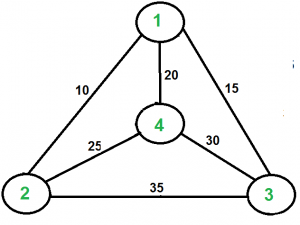
\includegraphics[width= 0.5\columnwidth]{fig/Euler12-300x225.png}
    \caption{Example of a full connected graph.}
    \label{fig:tsp_graph}
\end{figure}
\paragraph{Travels Salesman Problem Definition} Given a set of cities and distance between every pair of cities, the problem is to find the shortest possible route that visits every city exactly once and returns to the starting point.
\begin{lstlisting}[numbers=none]
Assume our graph is a two dimensional list:
g = [[(1, 10), (2, 15), (3, 20)], 
   [(0, 10), (2, 35),(3,25)],
   [(0, 15),(1,35),(3,30)],
   [(0,20),(1,25),(2,30)]]
g[0][0]=(1,10), means the edge between 0 and 1 with cost 10.
\end{lstlisting}
We show the above example in Fig.~\ref{fig:tsp_graph}.
\subsubsection{Analysis and Solution}
\paragraph{State Space} In TSP, we need to construct a list of vertices (\texttt{path}) and its total cost (\texttt{cost}) of all edges between as the state $s=(p, c)$, $p, c$ is short for path and cost respectively. A possible complete solution for path will have $n+1$ vertices which start with a vertex and end with the same, and $n-1$ vertices in between. Now, put together about constraints.
\begin{itemize}
    \item ``Visits every city exactly once'' means the first vertex will be a permutation of all cities, we get $n!$ combination (the last vertex does not matter).
    \item We have $n!$ possible states. We can further spot redundant states. For a cycle, it does not matter where it starts, it is always the same cycle. For convenience, we choose vertex $0$ as the starting path, and there will only be $n-1$ vertex to permutate with, making the size of the state space to $(n-1)!$. 
    \item We only care about the minimum cost, then any partial result that has cost larger than the  minimum cost of all known complete solution can be prunned. This is called \textit{Branch and bound} method, which is the extension of backtracking into the optimization problems.
\end{itemize}
\paragraph{Implementation} The implementation is a combination of \textbf{all paths} and \textbf{permutation}. We set the start vertex as $0$. \texttt{bused} will be a list of boolean to track if the element is in the path so that the first $n$ vertices will be a permutation. \texttt{cost} is used to record the current total cost. \texttt{mincost} tracks the minimum known cost of complete paths. The Python code is as follows:
\begin{lstlisting}[language=Python]
def tsp(g, cv, path, mincost, cost, bused, ans):
  '''
  cv represents the current node
  path: a list to track all vertices, we start from vertex 0, or we can use ordered set.
  '''
  if len(path) == len(g): # we can only choose 0
    cost += g[cv][0][1]
    if cost < mincost[0]:
      mincost[0] = cost
      ans[0] = path[::]
    return
  for v, c in g[cv]:
    # Bound the search by an estimation    
    if (not bused[v]) and (cost + c < mincost[0]):
        bused[v] = True
        path.append(v)
        cost += c
        tsp(g, v, path, mincost, cost, bused, ans)
        bused[v] = False
        path.pop()
        cost -= c
  return
\end{lstlisting}
In this example, we need constraint of permutation and the branch and bound, which is shown in line 14. The end condition of the problem is when we already have the first $n$ unique vertices, the last one must be the same as the start vertex. At this step, we track the \texttt{mincost} and save the path in \texttt{ans}. 

%%%%%%%%%%%%%%%%%%%%
\section{Knapsack Problem}
In this section we want to showcase more searching strategies applied in solving optimization problems: comparing backtracking and a chance to use best-first search strategy. 

\paragraph{Define Knapsack Problem} We are given $n$ items with a weight $w$ and a value vector $v$ and a knapsack with capacity $c$. Our goal is to choose a certain number of items with a total weight that is bounded by $c$.  Each item can be only used at most once.
\begin{lstlisting}[numbers=none]
For example,
c = 10
w = [5, 8, 3]
v = [45, 48, 35]

The best would be choosing item 1 and 3, with total weight of 8, and value of 80.
\end{lstlisting}
\subsubsection{Analysis} This is essentially a combination problem, we have to search a leaf node that is both feasible--bounded by capacity and optimal--has the largest value. 

To bound the search, we have to develop a heuristic function to estimate the maximum total value a branch can lead to. A simplest estimation is based on the total value of all items. At first in our case it will be  

A most closely heuristic function can come with \textbf{constraint relaxation}. What if we are allowed to get part of an item, so that we can fit the knapsack as full as possible. We can sort the items by their unit value, and take items in the order of decreasing unit values. Another bool vector is used to indicate if a certain item can be used or not. At first, all items are allowed, we can get an estimation of 92 in this case. For branches that decide not to take an item, that item is excluded using the bool vector.  We compare the estimation with the best found value, if the estimated value will never be better, then this branch will prunned. 
\subsubsection{Branch and Bound with Backtracking}
In this process, we only search in order of depth-first and bound by the estimation. The process is shown in Fig.~\ref{}. 
\begin{lstlisting}[language=Python]
class dfsBound:
  def __init__(self, c, v, w):
    self.best = 0 
    self.c = c
    self.v = v
    self.w = w
    self.n = len(v)
    self.items = [(-vi/wi, wi, i) for i, (vi, wi) in enumerate(zip(v, w))]
    self.items.sort(key=lambda x: x[0])
    self.dfs(0, self.estimate([True]*self.n), 0, 0,[True]*self.n)

  def estimate(self, blist):
    est = 0
    # use the v/w to estimate
    left = self.c
    j = 0
    n = len(blist)
    while left > 0 and j < n:
      ratio, wi, i = self.items[j]
      j += 1
      if not blist[i]:
        continue
      if left - wi >= 0: # use all
        est += -ratio * wi
        left -= wi
      else: # use part
        est += -ratio * (left)
        left = 0 
    print(est)
    return est
  
  def dfs(self, idx, est, val, cap, blist):
      if idx == self.n:
        self.best = max(self.best, val)
        return
      if cap + self.w[idx] <= c: # prune by constraint
        # bound by estimate
        if est > self.best:
          self.dfs(idx+1, est, val+self.v[idx], cap + self.w[idx], blist)

      # bound by estimate
      if est > self.best:
        blist[idx] = False
        nest =  self.estimate(blist)
        self.dfs(idx+1, nest, val, cap, blist) 
        blist[idx] = True
      return
\end{lstlisting}
\subsection{Branch and Bound with Best-First Search}
We can decide to expand branch that has the most optimistic estimation first, instead of blindly in order of depth-first,  hoping it will find a good enough global value with a higher bar to serve as a good start for the bounding; a higher bar will help us prune more worse branches faster. Supposedly, best-first search will guide us to find the optimal solution faster than backtracking, but we know it comes with higher cost in space usage. The process is shown in Fig.~\ref{}.
\begin{lstlisting}[language=Python]
import heapq
def bfs(c, v, w):
  # track val, cap, and idx is which item to add next
  q = [(-sum(v), 0, 0, 0)] # first simply use the sume of values as estimation
  n = len(v)
  best = 0
  while q:
    est, val, cap, idx = heapq.heappop(q)
    #print(est, val, cap, idx, q)
    if idx == n:
      best = max(best, val)
      continue
    est = -est
    nest = est - v[idx]

    if est > best: # bound, when all nodes are worse than the found best, prune
      if cap + w[idx] <= c: # prune by constraint
        heapq.heappush(q, (-nest, val+v[idx], cap + w[idx], idx+1))
      heapq.heappush(q, (-nest, val, cap, idx+1))
  return best
\end{lstlisting}


%%%%%%%%%summary%%%%%%%%%%%%%%%%%%%%%%
\subsection{Summary}

\paragraph{Backtracking Implementation} At first, backtracking might sounds scary and not many books out there did great job to ease it down. If we were to write down a standard template for backtracking, what are the elements? First, imagine that we are building and traverse a tree.
 \begin{enumerate}
     \item \textbf{State Vector $s$}: state vector is something we use to track the solution. In permutation and combination, it is \texttt{curr} and \texttt{path} in all paths problem. For the sudoku solver, this can be implemented in \texttt{unfilled} with the value and position. However, instead, it is easier to directly tracking it on the \texttt{board}.The state vector tells us the height of the tree, the candidates for each level is based on the constraint before. 
     \item \textbf{State Map and Candidates}: This is a good example of trading space for efficiency. The constraint of what candidates we have for current node depends on the previous state. We can get previous state by looking at the current result as in permutation in \texttt{curr} or the \texttt{board} in sudoku. However, each lookup took $O(n)$ time to complete. A smarter choice is to set aside another space with boolean or dictionary-like data structure to track the state along with the result data structure. Such as \texttt{used} in help of permutation and \texttt{row\_state}, \texttt{col\_state}, and \texttt{block\_state} to assist tracking the constraint in sudoku. Now to lookup if a candidate is possible we only need $O(1)$. 
 \end{enumerate}
 
 \paragraph{Time and Space Complexity} The time complexity analysis is straightforward which is the same as the DFS, $O(b^d)$. For the space, we have analyzed in the permutation example, however, it is important enough to summarize it here for emphasize. The backtracking techniques improves the space efficiency on the basis of DFS, which has $O(bd)$ using in two possible ways:
 \begin{enumerate}
     \item The backtracking mechanism itself that only generate one state a time on the fly, and not worrying about its sibling states brings the space complexity down to $O(d)$. 
     \item In our practice, we have seen another trick that we do not pass a new state to our recursive function each time. Instead, we make modification that takes $O(1)$ time complexity instead of $O(d)$ to copy the state, and undo the modification once we returned from the recursive call. This reduces the memory requirement to just one state vector and $O(d)$ actions to modify the state. This trick is both time and space saving.
 \end{enumerate}

\paragraph{Search Space Prunning Methods} We summarize the following three methods that can be potentially applied in a CSP or an optimization problem.  
\begin{enumerate}
     \item \textbf{Make Global Decision:} The backtracking works correctly if we do not update the each slot's candidates since initialization, we only make decision based on current node's validity. However, it would be more wise if each time we try an option, we check how this decision change remaining slots' candidates; if any of the remaining slots have zero candidates, we should better off stopping this shot and simply go to next option. 
    \item \textbf{Be Greedy about Ordering:} Each time we choose the spot that has the least number of candidates among the remaining spots list to update state with. This can be carried out with or without executing candidates updating for all remaining spots at each step. In our example of Suduku, we did update for all slots, but in some cases the cost might be too much or you just simply don't have enough time to write the code. 
    \item \textbf{*Symmetry:} Exploiting symmetry is another avenue for reducing combinatorial searches, prunning away partial solutions identical to those previously considered requires recognizing underlying symmetries in the search space. 
    \item \textbf{Branch and Bound:} Branch and bound is the idea of backtracking extended to optimization problems. We are minimizing a function with this useful property: A partial solution is pruned if its cost >= cost of best known complete solution.
\end{enumerate}

 
%  \paragraph{Backtracking VS Exhaustive Search} Backtracking helps in solving an overall problem by incrementally builds candidates {(implicit search tree)}. which is equivalent to finding a solution to the first sub-problem and then recursively attempting to resolve other sub-problems bases on the solution of the first sub-problem. Therefore, \textbf{Backtracking can be considered as a Divide-and-conquer method for exhaustive search.} Problems which are typically solved using backtracking technique have such property in common:  they can only be solved by trying every possible configuration and each configuration is tried only once(every node one time). A Naive exhaustive search solution is to generate all configurations and “pick” a configuration that follows given problem constraints. Backtracking however works in incremental way and \textbf{prunes} branches that can not give a result. It is an optimization over the exhaustive search where all possible(possible still with constraints) configurations are generated and tried. This comparison is called named as \textbf{Generating VS Filtering}. Backtracking can be viewed as a smart exhaustive search. 
 
%  Similarly, the difference between backtracking and DFS is the same. DFS is a searching technique applied on graph or tree data structures (more likely on explicit data structures). 
 
 There is an interesting questions. 
\begin{bclogo}[couleur = blue!30, arrondi=0.1,logo=\bccrayon,ombre=true]{As we explained DFS itself is an incomplete search technique, then why would backtracking search be complete?} 
\end{bclogo} 
 

%  \section{Bonus}
%  Generating combinations, permutation uniformly at random. 


\section{Exercises}
\subsection{Knowledge Check}

\subsection{Coding Practice}
\paragraph{Cycle Detection}
\begin{enumerate}
    \item 207. Course Schedule (medium)
\end{enumerate}

\paragraph{Topological Sort}

\paragraph{Connected Component}
\begin{enumerate}
    \item 323. Number of Connected Components in an Undirected Graph (medium).
    \item 130. Surrounded Regions(medium)
    \item 
\end{enumerate}

\paragraph{Mix}
\begin{enumerate}
    \item 210. Course Schedule II (medium, cycle detection and topological sort). 
\end{enumerate}

\paragraph{Backtracking}
\begin{enumerate}
\item 77. Combinations
\begin{lstlisting}
Given two integers n and k, return all possible combinations of k numbers out of 1 ... n.

Example:

Input: n = 4, k = 2
Output:
[
  [2,4],
  [3,4],
  [2,3],
  [1,2],
  [1,3],
  [1,4],
]
\end{lstlisting}

\item 17. Letter Combinations of a Phone Number
\begin{lstlisting}
Given a digit string, return all possible letter combinations that the number could represent.

A mapping of digit to letters (just like on the telephone buttons) is given below.

Input:Digit string "23"
Output: ["ad", "ae", "af", "bd", "be", "bf", "cd", "ce", "cf"].

Note:
Although the above answer is in lexicographical order, your answer could be in any order you want.
\end{lstlisting}

\item 797. All Paths From Source to Target (medium).

\item \textbf{37. Sudoku Solver (hard).}
Write a program to solve a Sudoku puzzle by filling the empty cells.

A sudoku solution must satisfy all of the following rules:
\begin{enumerate}
    \item Each of the digits 1-9 must occur exactly once in each row.
    \item Each of the digits 1-9 must occur exactly once in each column.
    \item Each of the the digits 1-9 must occur exactly once in each of the 9 3x3 sub-boxes of the grid.
\end{enumerate}
Empty cells are indicated by the character '.'.

\item %%%%%%%%%%%%%%%%%%%%%%Eight Queen%%%%%%%%%%%%%%%%%%%%%%%%%%%%%%%%%%%%%%%%%%%%%%%%%%%%
\subsection{Eight Queen}
\begin{figure}[!ht]
    \centering
    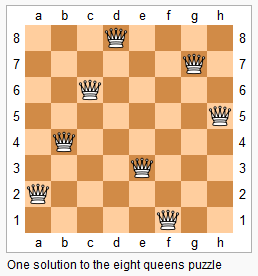
\includegraphics[width=0.6\columnwidth]{fig/8-queens.png}
    \caption{An examplary solution to the eight-queen problem.}
    \label{fig:solution_eight_queen}
\end{figure}
\paragraph{Eight Queen Problem  Definition}
Given a chessboard which is of size $8\times 8$, how many distinct ways to position eight queens on the chessboard such that no two queens threaten each other. According to the chess rules: a queen can move any step either horizontally, or vertically, or diagonally. Which is kind of similar to the rules of sudoku. There is another type of question which asks to return all distinct solutions. 
\begin{enumerate}
    \item Each row can only has one queen.
    \item Each column can only has one queen.
    \item Each diagonal can only has one queen.
\end{enumerate}
One examplary solution is shown in Fig.~\ref{fig:solution_eight_queen}. The problem can be extend to $n$-queen problem, which states on any size of $n\times n$ chessboard, how many ways to place $n$ queens that they are mutually non-attacking.  

\subsubsection{Analysis and Solution}
\paragraph{State Space} For the $n$ queens, it does not matter about the ordering; like the example, if we switch the positions of them, we will not get another solution. Therefore, it is a combination problem instead of permutation. For combination, we just care the position and for each position, it only differs if there is a queen or not (two choices), while not 9 (no queen plus any of the other queen). We have different ways to arrange these queens:
\begin{enumerate}
    \item No constraint: (1) if even no constraint of number of queens, for 64 positions, each has two states, this gives us $N=2^{64}$, (2) put the constraint of only 8 queens, we simply try to come out the possible combination of 8 queens on $8\times 8$ chessboard, it is going to be  $N = C_{64}^{8} =4426, 165,368$.
    \item Add constraint One: Now for the first row, we can have 8 different states, one and only one will have a queen, same for any other rows followed by. We end up with $N=8^8$.
    \item Add constraint Two: If each column can only have one queen, then for the first row, it will have 8 possible states, while the second can only have 7, thus making $N=8!$, which is less that $10^6$ and is possible for programs to run. 
\end{enumerate}
\begin{figure}[!ht]
    \centering
    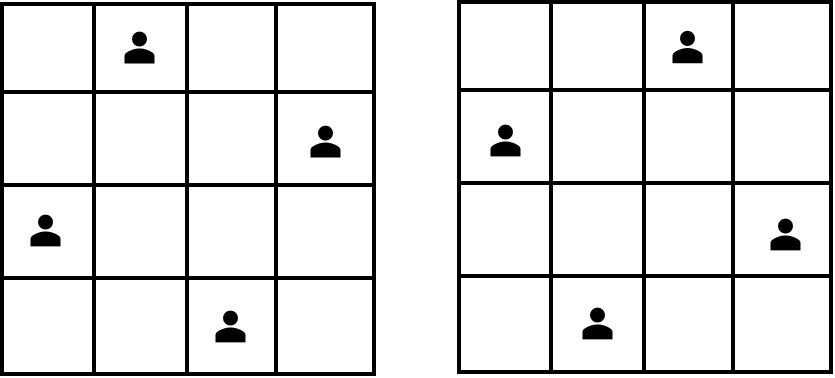
\includegraphics[width=0.6\columnwidth]{fig/n_queen_four.png}
    \caption{Solutions shown of $4 \times 4$ chessboard}
    \label{fig:n_queen_four}
\end{figure}
The above analysis reveals that our state vector should be of size of the total number of rows, $S=[None]*8$, with the index to represent the row in the chessboard, and the value to be an integer from 0 to n-1 to track the column that has a queen. It is similar to a permutation problem. For $4\times 4$ board, we have the following two solutions, represented with $S$, it is $S=[1, 3, 0, 2], [2, 0, 3, 1]$.  Therefore, our search tree will be of height 8. For edges which represent possible candidate, we can have two ways to generate candidates: (1) easy one that we iterate through all 9 columns for each row and we just need to validate each candidate through \texttt{assist\_state\_tracker}. (2) generate candidate based on previous state vector $s$. 

\paragraph{Implementation} 
\begin{figure}[!ht]
    \centering
    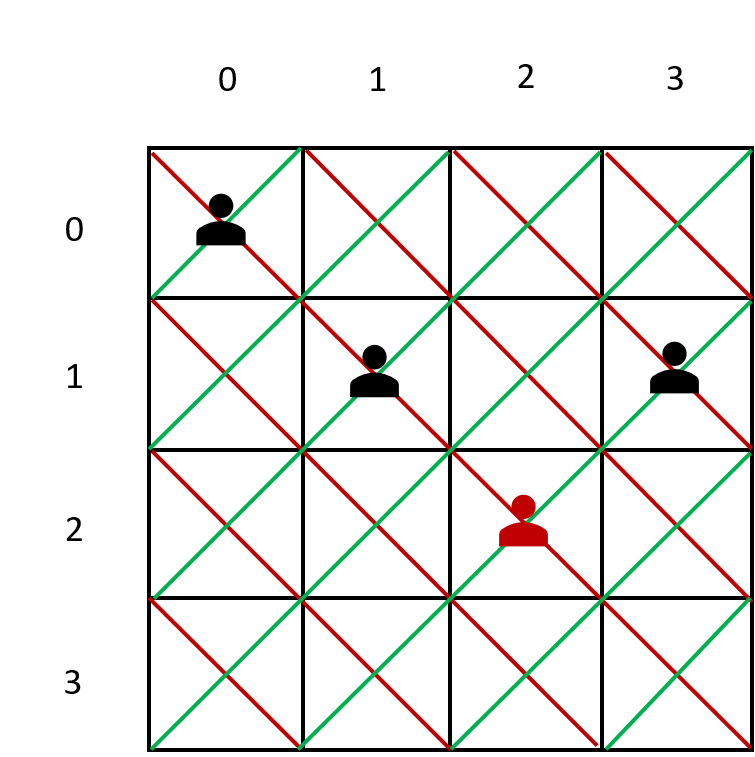
\includegraphics[width=0.6\columnwidth]{fig/n_queen_diag.png}
    \caption{Caption}
    \label{fig:my_n_queen_diag}
\end{figure}

We use \texttt{n\_queen} a list whose index indicates the row of the chessboard and the value represents the column that we put the queen in. It starts as an empty list and with a possible maximum length of $n$. Because in the backtracking, each level represents the row, thus we do not need to track the row state. We need to have \texttt{col\_state} to track if a column has a queen already. As indicates in Fig.~\ref{fig:my_n_queen_diag}, for each possible position, we need to check the left and right diagonal if a queen already put there. Here, we use two lists \texttt{left\_diag} and \texttt{right\_diag} to track them. For position $(r, c)$, the position at the \texttt{left\_diag} will be (r-1, c-1), (r+1, c+1), the rule is bit hidden that r-c = (r-1)-(c-1) = (r-2)-(c-2). For the \texttt{right\_diag}, it will be (r-1, c+1), (r+1, c-1), thus the same diag has the same value of (r+c). The implementation is as follows:
\begin{lstlisting}[language=Python]
def solveNQueens(self, n):
    """
    :type n: int
    :rtype: List[List[str]]
    """
    # queen can move: vertically, horizontally, diagonally 
    col_state = [False]*n
    #diag =[False]*n
    left_diag = [False]* (2*n-1) # x+y -> index
    right_diag = [False]* (2*n-1) # x+(n-1-y) ->index
    n_queen = [] # to track the positions
    ans = []
    board = [['.' for i in range(n)] for j in range(n)] #initialize as '.' we can try to flip
    def collect_solution():
        board = [['.' for i in range(n)] for j in range(n)] 
        for i, j in enumerate(n_queen):
            board[i][j] = 'Q'
            
        for i in range(n):
            board[i] = ''.join(board[i])
        return board
    
    def is_valid(r, c):
        return not (col_state[c] or left_diag[r+c] or right_diag[r+(n-1-c)])
      
    def set_state(r, c, val):
        col_state[c] = val
        #diag[abs(r-c)] = val
        left_diag[r+c] = val
        right_diag[r+(n-1-c)] = val
        
    def backtrack(n_queen, k):
        if k == n: # a valid result
            ans.append(collect_solution())
            return
        # generate candidates for kth queen
        for col in range(n):
            if is_valid(k, col):
                set_state(k, col, True)
                n_queen.append(col)
                backtrack(n_queen, k+1)
                set_state(k, col, False)
                n_queen.pop()
            
    backtrack(n_queen, 0)
    return ans
\end{lstlisting}

There is another way to generate candidates based on \texttt{n\_queen}. At the first row, we have candidates of [0, 1, 2, 3]. Assume we choose 1 here, and at row 1, we generate candidates based on previous rows. We remove the ones on the diagnal and columns. The code is implemented as:
\begin{lstlisting}[language=Python]
def solveNQueens2(self, n):
  """
  :type n: int
  :rtype: List[List[str]]
  """
  n_queen = [] # to track the positions
  ans = []
  board = [['.' for i in range(n)] for j in range(n)] #initialize as '.' we can try to flip
  def collect_solution():
      board = [['.' for i in range(n)] for j in range(n)] 
      for i, j in enumerate(n_queen):
          board[i][j] = 'Q'

      for i in range(n):
          board[i] = ''.join(board[i])
      return board
      
  def generate_candidate(n_queen, k, n):
    if k == 0: #the first row, then the candidates row is all columns
      return set([i for i in range(n)])
    # generate candidate in kth level based on previous levels
    candidates = set([i for i in range(n)])
    for r, c in enumerate(n_queen):
      if c in candidates:
        candidates.remove(c)
      c1 = c-(k-r)
      if c1 >=0 and c1 in candidates:
        candidates.remove(c1)
      c2 = c+(k-r)
      if c2 < n and c2 in candidates:
        candidates.remove(c2)
    return candidates

  def backtrack(n_queen, k):
      if k == n: # a valid result
          ans.append(collect_solution())
          return
      # generate candidates for kth queen
      candidates = generate_candidate(n_queen, k, n)
      for c in candidates:
          n_queen.append(c)
          backtrack(n_queen, k+1)
          n_queen.pop()

  backtrack(n_queen, 0)
  return ans
\end{lstlisting}
\paragraph{Symmetry}
\begin{figure}[!ht]
    \centering
    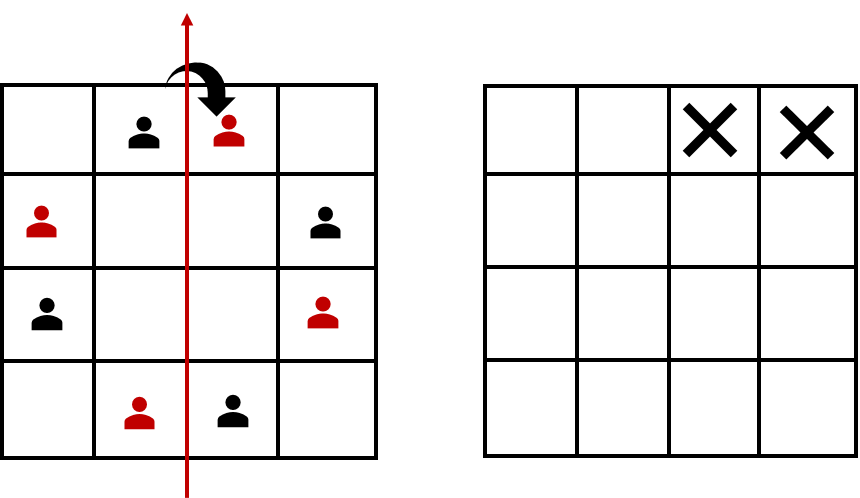
\includegraphics[width=0.6\columnwidth]{fig/n_queen_symmetry.png}
    \caption{Mirroring can cut the search space into half.}
    \label{fig:n_queen_symmetry}
\end{figure}
\begin{figure}[!ht]
    \centering
    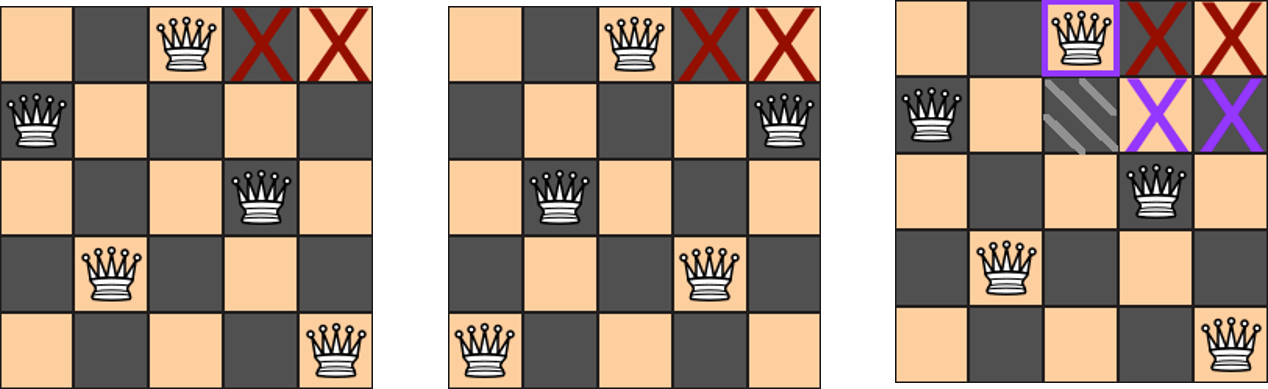
\includegraphics[width=0.6\columnwidth]{fig/n_queen_oddPicture1.png}
    \caption{Mirroring can cut the search space into half.}
    \label{fig:n_queen_odd}
\end{figure}
\url{https://www.aaai.org/Papers/AAAI/2006/AAAI06-257.pdf}.  Start from  an easy one, we can observe that we can obtain the second solution of $4\times 4$ chessboard by flipping around the first around  the red axis. Assume our first solution is $S=[1, 3, 0, 2]$. We represent the $S=[a_0, a_1, a_2, a_3]$. Now the mirroring relation can be represented as $m_i+a_i=n-1$, thus $m_i=n-1-a_i$. If n is even, then at the first level of backtracking, we can elimiate the second half of candidates, which cut of search cost into half of the previous. If we just need to count the total number of distinct solutions, we can just double the number we find. The process is shown in Fig.~\ref{fig:n_queen_symmetry}. For odd one, for the middle spot at the first row, if we follow the same rule as in the even $n$, some solutions shown in follows will be doubled. So we need to distinguish the middle spot situation in odd $n$ case. If we place a queen in the middle spot of the first row, then for the following $n-1$ rows, no one will be in the middle column any more. For the second row, we can eliminate the other half of candidates on the right side as shown in Fig.~\ref{fig:n_queen_odd}. Our code become:
\begin{lstlisting}[language=Python]
def solveNQueensSymmetry(n):
  """
  :type n: int
  :rtype: List[List[str]]
  """
  n_queen = [] # to track the positions
      
  def generate_candidate(n_queen, s, k, n):
    if k == s: #apply symmetry
      candidates = set([i for i in range(n//2)])
    else:
      candidates = set([i for i in range(n)])

    for r, c in enumerate(n_queen):
      if c in candidates:
        candidates.remove(c)
      c1 = c-(k-r)
      if c1 >=0 and c1 in candidates:
        candidates.remove(c1)
      c2 = c+(k-r)
      if c2 < n and c2 in candidates:
        candidates.remove(c2)
    return candidates

  def backtrack(n_queen, s, k, ans):
      '''add s to track the start depth'''
      if k == n: # a valid result
          ans += 1
          return ans
      # generate candidates for kth queen
      candidates = generate_candidate(n_queen, s, k, n)
      for c in candidates:
          n_queen.append(c)
          ans = backtrack(n_queen, s, k+1, ans)
          n_queen.pop()
      return ans
    
  # deal with the left half of the first row
  ans = 0

  ans += backtrack(n_queen, 0, 0, 0)*2
  
  # deal with the left half of the second row
  if n%2 == 1:
    n_queen = [n//2]
    ans += backtrack(n_queen, 1, 1, 0)*2
  return ans
\end{lstlisting}
\end{enumerate}
\end{document}\paragraph{Alternative: Swapping Method}   

